\documentclass[a4j,titlepage]{jarticle}
\usepackage[dvipdfmx]{graphicx}
\usepackage{ascmac}
\usepackage{float}
\usepackage{amssymb}%にやりイコールを使う
\usepackage{multirow}
\usepackage{multicol}
%\usepackage{color}

\begin{document}

\title{2022 年度 3 回生前期学生実験 HW  \\ \bf team02 機能設計仕様書 植田健斗担当分}
% ↓ここに自分の氏名を記入
\author{氏名:植田健斗 入学年度:2020年度 学籍番号:1029-32-6498}
\西暦
\date{提出期限:4月15日18時 提出日: \today} % コンパイル時の日付が自動で挿入される
\maketitle
\newpage

\section{実験環境}
導入課題の実験で使用したボードやCADツールを以下に記す。

\begin{itemize}
\item ボード \\Rapid Prototyping Kit PowerMedusa \\ MU500-RXSET01(MU500-RX, MU500-RK, MU500-7SEG) \\「」の番号の書かれたボードを使った。  
\item CADツール \\ Quartus Prime Version 17.1.0 Build 590 10/25/2017 SJ Lite Edition
\end{itemize}

\section{全体のコンポーネント分割方法}

%\subsection{設計する回路の仕様}
%\subsection{設計の詳細}
%\subsubsection{ピン割当て}
%\subsection{正しく動作したか}
それぞれの機能を持った回路ごとにモジュール分割した。
各回路につけたファイル名は図\ref{moduleSplit0422}に示した通りである。(次の章の図\ref{rolesDivision0422}でまとめてある。)


\begin{figure}[H]
    \begin{center}
    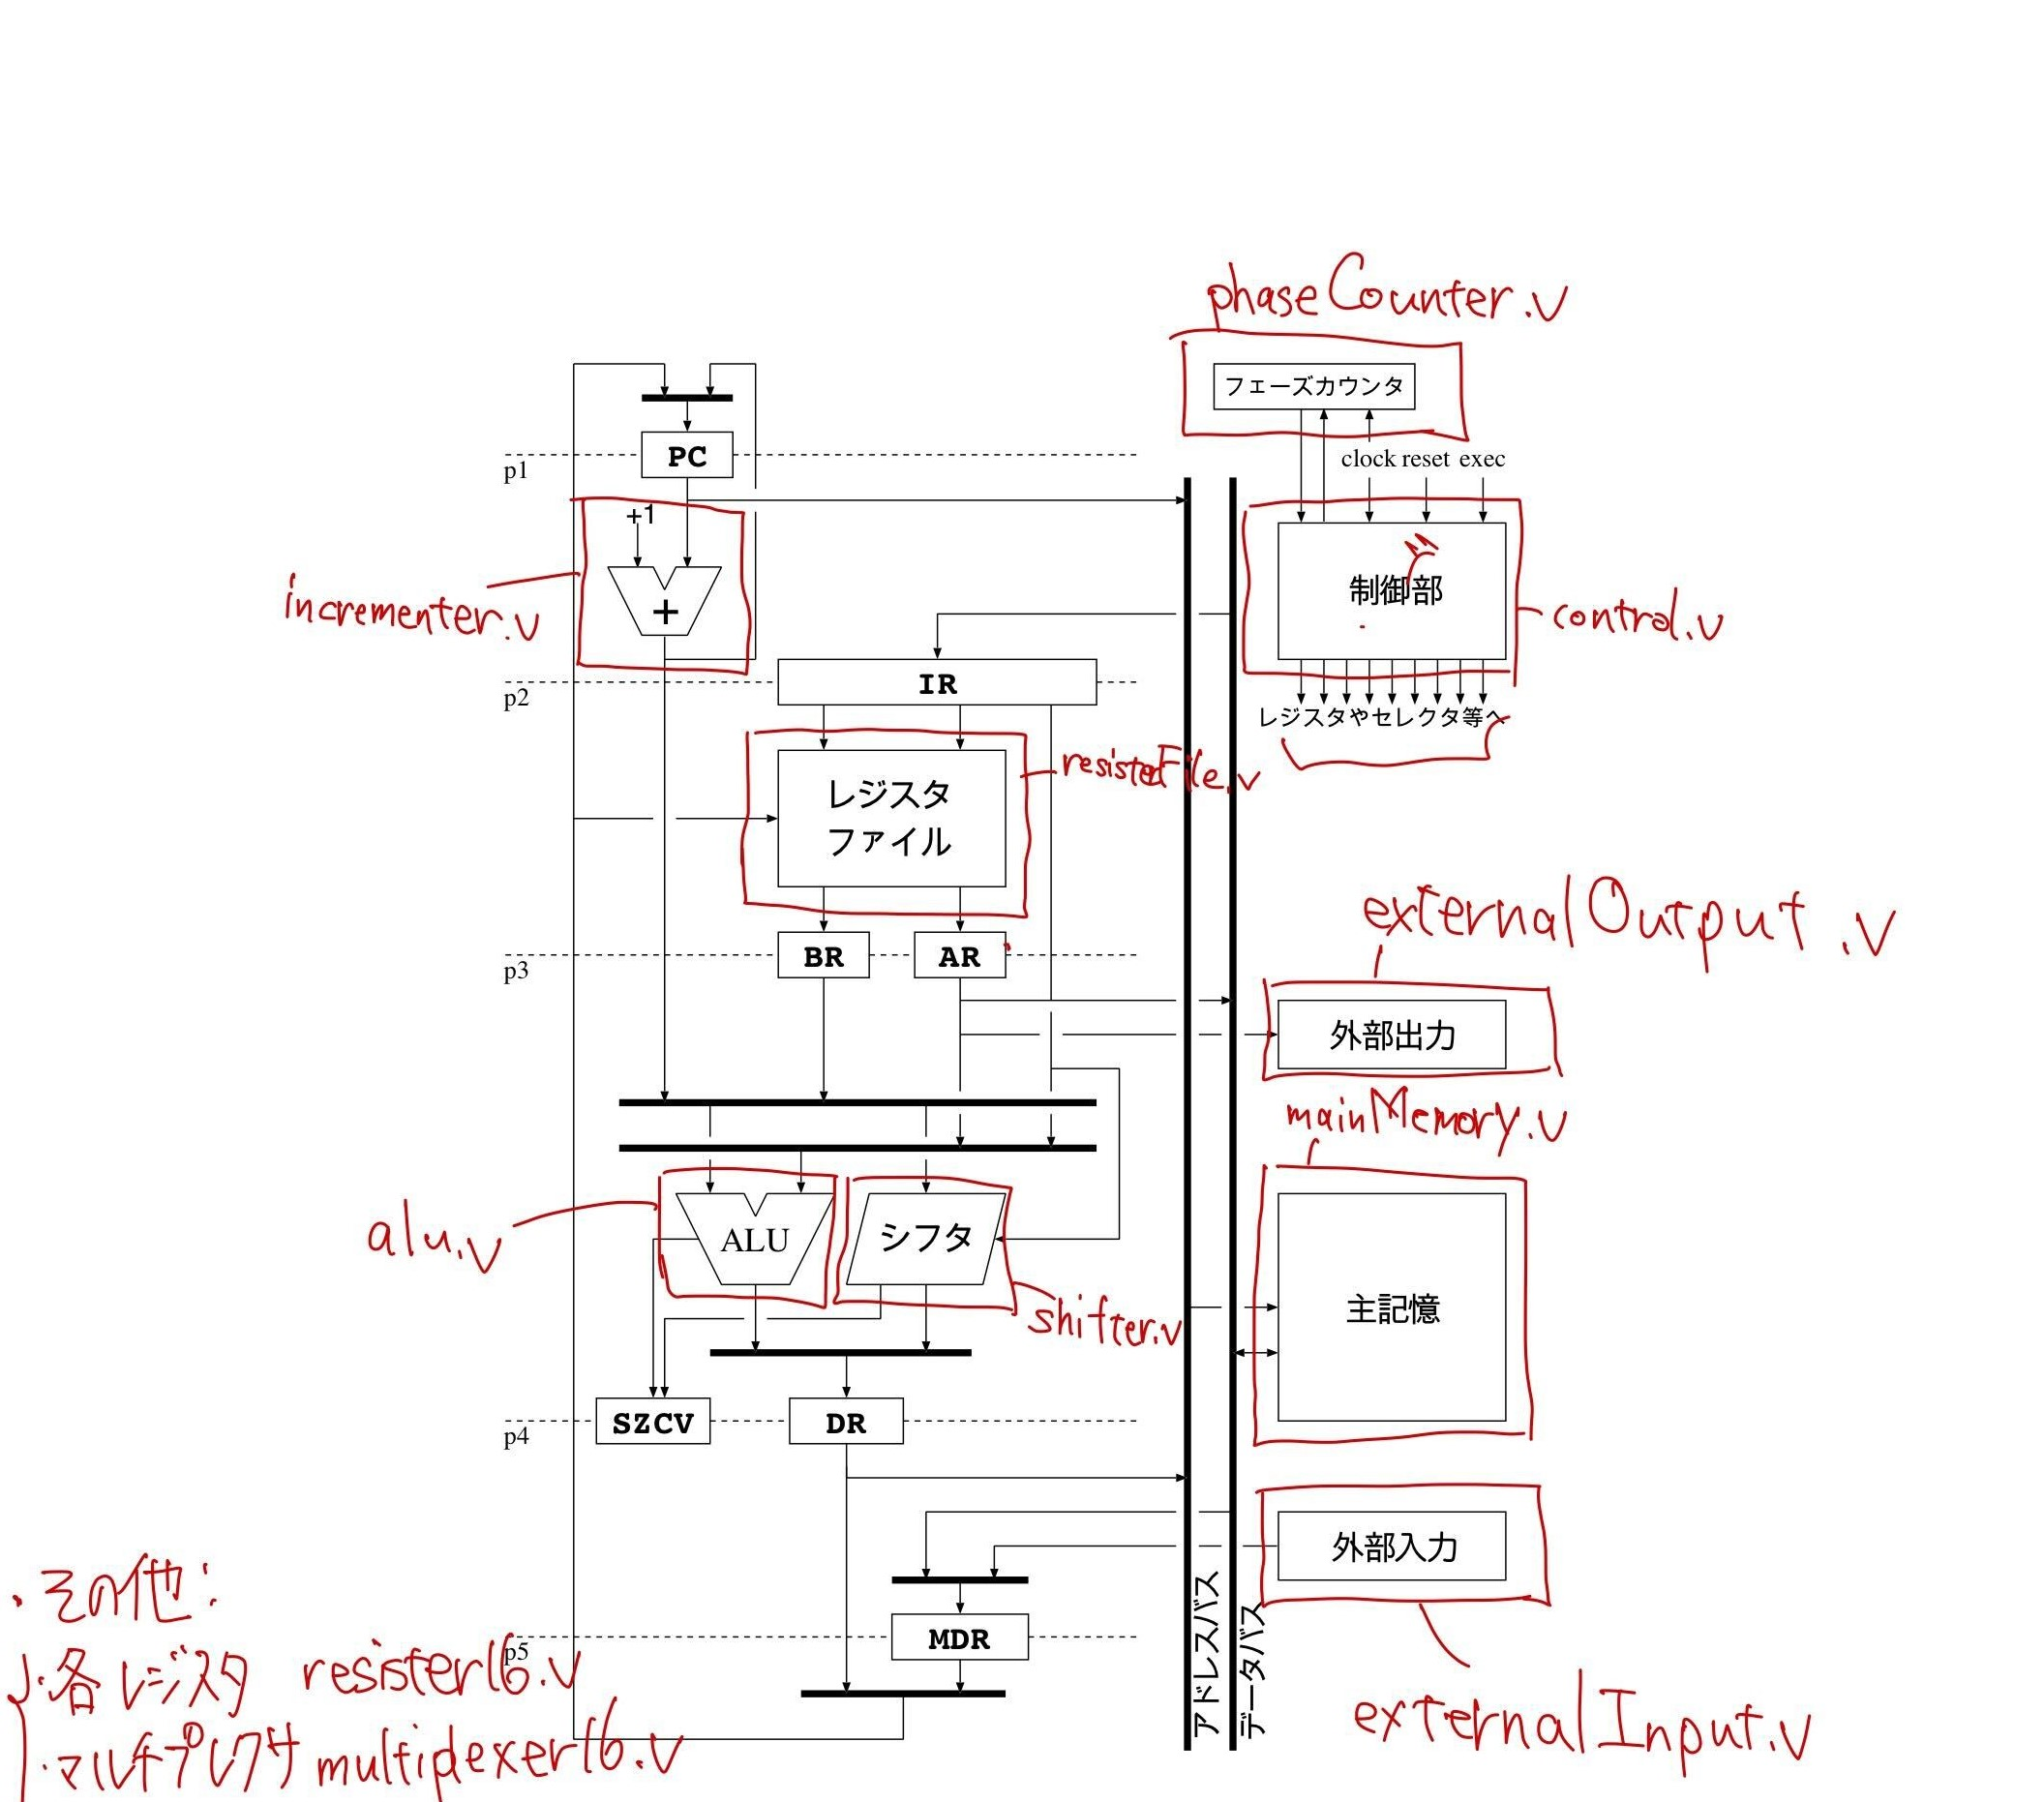
\includegraphics[scale = 0.22]{moduleSplit0422.jpg}
    \end{center}
    \caption{モジュール分割の方法の図}
    \label{moduleSplit0422}
\end{figure}

役割分担の表を以下の図\ref{rolesDivision0422}に示す。

\begin{figure}[H]
    \begin{center}
        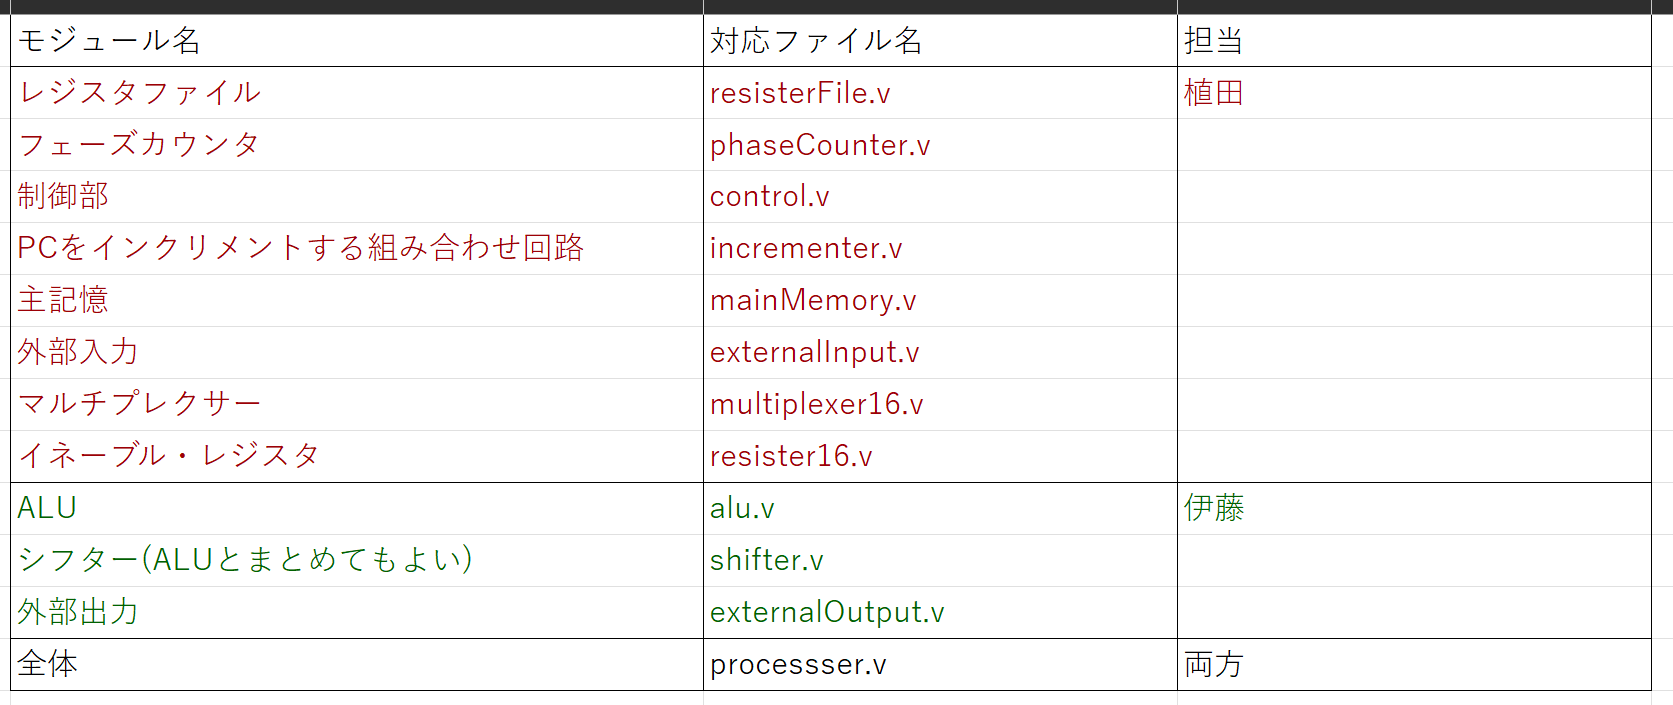
\includegraphics[scale = 0.5]{rolesDivision0422.png}
    \end{center}
    \caption{役割分担(4月22日時点)}
    \label{rolesDivision0422}
\end{figure}


\section{設計を担当したコンポーネント}
設計を担当したコンポーネントは以下である。
\begin{itemize}
    \item レジスタファイル(registerFile.v)
    \item フェーズカウンタ(phaseCounter.v)
    \item 制御部(control.v)
    \item PCをインクリメントする組み合わせ回路(incrementer.v)
    \item 主記憶(mainMemory.v)
    \item 外部入力(externalinput.v)
    \item マルチプレクサー(multiplexer.v)
    \item イネーブル・レジスタ(register16.v)
    \item 全体(processor.bdf)
\end{itemize}



\section{レジスタファイル(registerFile.v)}

\subsection{回路の外部仕様}
ファイルの入出力は以下の表\ref{registerFileIO}のようになる。

\begin{table}[H]
    \caption{aの表す16進数の数字とaとoutの論理関係}
    \label{aとoutの論理関係}
    \begin{center}
    \begin {tabular}{|c|c|c|} \hline
    名前(ファイル名)& input & input説明 & output & outputの説明 \\ \hline \hline
    \multirow{8}{*}{レジスタファイル(registerFile.v)}  & Rs[2:0] & 命令中のRs・Raをあたえる。 & AR[15:0] & Rs番目のレジスタの値を読み込む。 \\ \hline
                                                     & Rd[2:0] & 命令中のRd・Rbをあたえる。 & BR[15:0] &  \\ \cline{2-3}
                                                     & regWrite &  &  &  \\ \cline{2-3}
                                                     & writeData[15:0] &  &  &  \\ \cline{2-3}
                                                     & writeRegister[2:0] &  &  &  \\ \cline{2-3}
                                                     & clock &  &  &  \\ \cline{2-3}
                                                     & reset &  &  &  \\ \cline{2-3}
                                                     & changeEnable &  &  &  \\ \cline{2-3}
                                                     &  &  &  &  \\ \cline{2-3}
                                                     &  &  &  &  \\ \cline{2-3}
                                                     &  &  &  &  \\ \hline
    \end {tabular}
    \end{center}
    \end{table}




\subsection{回路の内部仕様}


\end{document}